\section{ThingSat}
\label{sec:case-study}

\subsection{Overview}
% \paragraph*{Mission Goal:} in-orbit observation of glaciers in Europe and in Polynesia.
% \paragraph*{Approach}: rent "rack" space as payload on a CubeSat (SatRevolution).

%----important
% citation --> Antenna : technical report
%----secondary
% Stork mission (404) : https://web.archive.org/web/20210420173051/https://satrevolution.com/products/stork-mission/
%in comparison to other project a GW in the sky not just a ping
% Sat-IoT

% Most of the earth’s surface lack of terrestrial networks. These zones include
% populated areas that necessitate technologies to permit communication with more
% connected areas, enable scientists to have networks in wild areas (e.g. Polar
% zones and oceans) to support their research, monitor isolated beacons and
% prevent of risks. Solutions have been developed in the last decades, notably the
% LoRa technology, that facilitate a long range communication with a low power
% consumption for IoT (Internet of things). 

The goal of the ThingSat project is to design a communication payload
constituted of an electronic board of several LoRa transmitters and a patch
antenna operating in (868MHz, 2.4GHz). It is a guest payload of a LEO (Low Earth
Orbit) shared 3U CubeSat - STORK-1 of the polish start-up
\href{https://www.satrevolution.com/}{SatRevolution} launched on a near-polar
orbit at an altitude of 520 km.
Such CubeSats offer payload slots ranging from 0,25U slots, to 0,5U slots or a 1U slot, and their expected lifetime is 5 years.
The CubeSat launched January 2022. 

% OA: vérifier le near-polar orbit, SSO, ...

The mission aims to benchmark the LoRa links over a very long distance (520 km)
for several frequency bands and demonstrate the effectiveness of that technology
in the context of space-ground communication.

% LEO orbit polar circular
% DtS-IoT (Direct-to-satellite)

This project can be adapted to a wide range of use cases, for players as varied
as Earth science researchers (e.g. Ocean levels, melting of glaciers, pirate
fishing...) and companies with widely dispersed objects (e.g. theMonitoring of
tank ships). 
% The transmitters and the antenna will connect the on ground
% isolated objects and beacons and ensure their re-synchronization by distributing
% a secure time base without the GPS. 

% OA: mentionner les partenaires

\paragraph*{High-level overview of Segments}

As illustrated in figure \ref{fig:thingsat-comm}, the Thingsat payload may act in turns as 
\begin{enumerate}
    \item either a Sat-IoT end-device (ED) that will send Lora frames to existing terrestrial LoRaWAN networks
    \item or an in-orbit sniffer of Lora traffic
    \item or a satellite store-and-forward LoRa gateway
\end{enumerate}

In the third scenario, the satellite stores data received from ground
stations(GS)/EDs and deliver it when destination GSs/EDs are covered by the
footprint of the satellite. The % \href{https://gricad-gitlab.univ-grenoble-alpes.fr/thingsat/public/-/tree/master/cubesat_mission/mission_scenario}{Thingsat missions}
are detailed on the Thingsat git repository. 

% annoter la figure avec des numéro pour bien la séquence des messages

\begin{figure}[t]
    \centering
    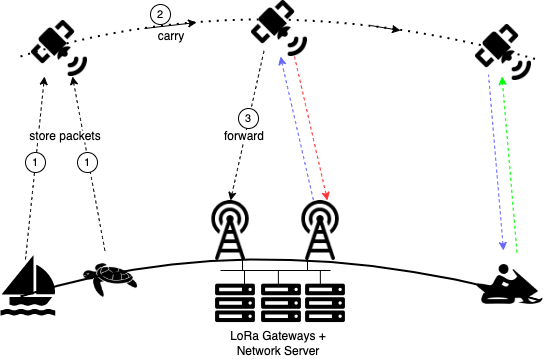
\includegraphics[width=0.5\textwidth]{Figures/thingsat-dtn.png}
    \caption{ThingSat in-orbit communication patterns.}
    \label{fig:thingsat-comm}
\end{figure}

\subsection{Distributed System Architecture}
\paragraph*{Ground Segment Description}
\paragraph*{Space Segment Description}

% il y a aussi la voie descendante de SR à mettre
% antenna : patch, circular polarization right hand ? (voir papier Tan à mettre en rapport)

% https://gricad-gitlab.univ-grenoble-alpes.fr/thingsat/public/-/blob/master/cubesat_mission/README.md#lora-communication-payload-onboard-of-stork-1-mission

The board embeds one \href{https://www.semtech.com/products/wireless-rf/lora-gateways/sx1302}{Semtech SX1302 concentrator} for communications on the 863-870 MHz 
band and one \href{https://www.semtech.com/products/wireless-rf/24-ghz-transceivers/sx1280}{Semtech SX1280 transceiver} for communications on the 2400-2500 MHz band. 
The firmware of the two STM32 MCUs is developed with \href{https://github.com/RIOT-OS/RIOT}{RIOT OS}.

image de la board ?

\paragraph*{Control Segment} % Francisco: not sure if its the right name
\paragraph*{OBC \& Payload Communication Bus}
\paragraph*{Payload Description}: tenant status, energy budget, on time etc.
% - OBC -> SatRev controlled
% - Payload -> Full Control

\subsection{Communication Characteristics Overview}
\paragraph*{link-budget Mission Control}: delivering and communicating mission
files, delivering software updates, latency, etc.
\paragraph*{link-budget Mission}: communication between OBC and Payload, payload
active time for communication with ground segments.

\subsection{Software Updates Requirements}
\paragraph*{What needs updates}: ?
\paragraph*{Why?}: timeline for deployment, CoVID context, etc. making it impossible
to deliver a fully functional device in time. Need to update the firmware remotely
and in orbit.
\paragraph*{Communication Chain}: how are new firmware, payloads delivered,
who has access, etc..

